\documentclass[12pt,ngerman,a4paperpaper,]{paper}
\usepackage{lmodern}
\usepackage{amssymb,amsmath}
\usepackage{ifxetex,ifluatex}
\usepackage{fixltx2e} % provides \textsubscript
\ifnum 0\ifxetex 1\fi\ifluatex 1\fi=0 % if pdftex
  \usepackage[T1]{fontenc}
  \usepackage[utf8]{inputenc}
\else % if luatex or xelatex
  \ifxetex
    \usepackage{mathspec}
  \else
    \usepackage{fontspec}
  \fi
  \defaultfontfeatures{Ligatures=TeX,Scale=MatchLowercase}
\fi
% use upquote if available, for straight quotes in verbatim environments
\IfFileExists{upquote.sty}{\usepackage{upquote}}{}
% use microtype if available
\IfFileExists{microtype.sty}{%
\usepackage{microtype}
\UseMicrotypeSet[protrusion]{basicmath} % disable protrusion for tt fonts
}{}
\usepackage[unicode=true]{hyperref}
\hypersetup{
            pdftitle={Was ist los?},
            pdfauthor={Halbjahresarbeit 2016/2107 von Jaro Habiger},
            pdfborder={0 0 0},
            breaklinks=true}
\urlstyle{same}  % don't use monospace font for urls
\ifnum 0\ifxetex 1\fi\ifluatex 1\fi=0 % if pdftex

\usepackage[shorthands=off,main=]{babel}
\else
  \usepackage{polyglossia}
  \setmainlanguage[]{}
\fi
\usepackage{polyglossia}
\setdefaultlanguage{german}
\usepackage[]{biblatex}
\addbibresource{bib.bib}
\usepackage{listings}
\usepackage{graphicx,grffile}
\makeatletter
\def\maxwidth{\ifdim\Gin@nat@width>\linewidth\linewidth\else\Gin@nat@width\fi}
\def\maxheight{\ifdim\Gin@nat@height>\textheight\textheight\else\Gin@nat@height\fi}
\makeatother
% Scale images if necessary, so that they will not overflow the page
% margins by default, and it is still possible to overwrite the defaults
% using explicit options in \includegraphics[width, height, ...]{}
\setkeys{Gin}{width=\maxwidth,height=\maxheight,keepaspectratio}
\IfFileExists{parskip.sty}{%
\usepackage{parskip}
}{% else
\setlength{\parindent}{0pt}
\setlength{\parskip}{6pt plus 2pt minus 1pt}
}
\setlength{\emergencystretch}{3em}  % prevent overfull lines
\providecommand{\tightlist}{%
  \setlength{\itemsep}{0pt}\setlength{\parskip}{0pt}}
\setcounter{secnumdepth}{5}
% Redefines (sub)paragraphs to behave more like sections
\ifx\paragraph\undefined\else
\let\oldparagraph\paragraph
\renewcommand{\paragraph}[1]{\oldparagraph{#1}\mbox{}}
\fi
\ifx\subparagraph\undefined\else
\let\oldsubparagraph\subparagraph
\renewcommand{\subparagraph}[1]{\oldsubparagraph{#1}\mbox{}}
\fi

% set default figure placement to htbp
\makeatletter
\def\fps@figure{htbp}
\makeatother


\title{Was ist los?}
\providecommand{\subtitle}[1]{}
\subtitle{Erhebung und Visualisierung von empirischen Daten verschiedener
Internet-Zeitungen}
\author{Halbjahresarbeit 2016/2107 von \emph{Jaro Habiger}}
\date{}

%%%%%%%%%%%%%%%%%%%%%%%%%%%%%%%%%%%%%%%%%%%%%%%%%%%%%%%%%%%%%%%%%%%%%%%%%%%%%%%%%%%%%%%%%%%%%%%
\usepackage{todonotes}

\usepackage{titletoc,tocloft}
\setlength{\cftsubsecindent}{2cm}
\setlength{\cftsubsubsecindent}{4cm}
\dottedcontents{section}[1.5em]{}{1.3em}{.6em}

\usepackage{xcolor}
\lstdefinelanguage{javascript}{
  morekeywords={typeof, new, true, false, catch, function, return, null, catch, switch, var, if, in, while, do, else, case, break},
  morecomment=[s]{/*}{*/},
  morecomment=[l]//,
  morestring=[b]",
  morestring=[b]'
}
\lstset{
    basicstyle=\ttfamily,
    numbers=left,
    keywordstyle=\color[rgb]{0.13,0.29,0.53}\bfseries,
    stringstyle=\color[rgb]{0.31,0.60,0.02},
    commentstyle=\color[rgb]{0.56,0.35,0.01}\itshape,
    numberstyle=\footnotesize,
    stepnumber=1,
    numbersep=5pt,
    backgroundcolor=\color[RGB]{248,248,248},
    showspaces=false,
    showstringspaces=false,
    showtabs=false,
    tabsize=2,
    captionpos=b,
    breaklines=true,
    breakatwhitespace=true,
    breakautoindent=true,
    escapeinside={\%*}{*)},
    linewidth=\textwidth,
    basewidth=0.5em,
    language=javascript,
}

\renewcommand{\figureshortname}{Abb.}

\renewcommand{\autocite}{\cite}
\renewcommand{\bibliography}{\printbibliography}
%%%%%%%%%%%%%%%%%%%%%%%%%%%%%%%%%%%%%%%%%%%%%%%%%%%%%%%%%%%%%%%%%%%%%%%%%%%%%%%%%%%%%%%%%%%%%%%

\begin{document}
\maketitle
\thispagestyle{empty}

\newpage
\thispagestyle{empty}
{
\setcounter{tocdepth}{3}
\tableofcontents
}
\newpage
\setcounter{page}{1}
% pandoc-xnos: macro to create a caption without a prefix
\makeatletter
\long\def\@makenoprefixcaption#1#2{
  \vskip\abovecaptionskip
  \sbox\@tempboxa{#2}
  \ifdim \wd\@tempboxa >\hsize
    #2\par
  \else
    \global \@minipagefalse
    \hb@xt@\hsize{\hfil\box\@tempboxa\hfil}
  \fi
  \vskip\belowcaptionskip}
\makeatother

% pandoc-fignos: save original macros
\makeatletter
\let\@oldmakecaption=\@makecaption
\let\oldthefigure=\thefigure
\let\oldtheHfigure=\theHfigure
\makeatother

% pandoc-fignos: environment disables figure caption prefixes
\makeatletter
\newcounter{figno}
\newenvironment{no-prefix-figure-caption}{
  \let\@makecaption=\@makenoprefixcaption
  \renewcommand\thefigure{x.\thefigno}
  \renewcommand\theHfigure{x.\thefigno}
  \stepcounter{figno}
}{
  \let\thefigure=\oldthefigure
  \let\theHfigure=\oldtheHfigure
  \let\@makecaption=\@oldmakecaption
  \addtocounter{figure}{-1}
}
\makeatother

\section{Idee}\label{idee}

\begin{itemize}
\tightlist
\item
  ich -\textgreater{} Programmieren
\item
  ich -\textgreater{} Zeitung -\textgreater{} klo -\textgreater{}
  spiegel -\textgreater{} wortwolke
\item
  ich -\textgreater{} politisch
\item
  eig TR website
\item
  wie funktionieren Zeitungen?
\item
  anschpruchsvoll
\item
  -\textgreater{} was denken medien
\item
  anwendungsmöglichkeinten
\end{itemize}

Relativ schnell war mir klar, das ich mich mit Datenvisualisierung
beschäftigen will. Anfangs war allerdings nicht ganz klar, welchen
Datensatz ich auf welche Aspekte hin untersuchen will. Eines tages nahm
ich dann eine Ausgabe des Spiegels zur Hand und sah auf der ersten seite
eine sogenannte Wortwolke. Diese form der Darstellungy

Am Anfang dieser Halbjahresarbeit stand die Idee, die aktuelle
Nachrichtenlage visuell sichtbar zu machen. Dies sollte möglichst
intuitiv und aufschlussreich sein. Außerdem

\section{1 Tasse Tee}\label{tasse-tee}

Da nun die Daten fertig live in eine Datenbank ``fließen'' kann der
Interessante teil beginnen: Die Visualisierung und Auswertung. Hierbei
können verschiedenen Analysen vorgenommen werden. All diese sind nicht
trivial, da immer versucht erden muss aus einem Feließtext, also einem
Format, mit dem Computer eigentlich nichts anfangen können Informationen
zu gewinnen und zu veranschaulichen. Hierbei ist eine besondere
Herausforderung, dass dies alles passieren muss, obwohl der Computer
eigentlich über kein versändniss von ``Sinn'' verfügt. Aus diesem Grund
müssen statistische Verfahren als Hilfsmittel zur Hand gezogen werden,
die es dem Menschen, der die Daten letztenendes interpretiert
ermöglichen Informationen aus der Datenmenge zu ziehen.

\begin{itemize}
\tightlist
\item
  Generelle Gedanken
\item
  Vortrag über spon
\item
  Teilweise sehr schwierig zu verstehen -\textgreater{} Datenstrukturen
  ineinander umwandeln: wenig greifbar
\end{itemize}

\section{Die Auswahl der Zeitungen}\label{die-auswahl-der-zeitungen}

\begin{enumerate}
\def\labelenumi{\arabic{enumi}.}
\tightlist
\item
  Spiegel.de
\item
  Bild.de
\item
  Focus.de
\item
  Welt.de
\item
  Zeit.de
\item
  Faz.net
\end{enumerate}

AGOF November 2014: Die Top 50 der Nachrichten-Websites Unique User
November vs.~Oktober 1 Bild.de 16,91 -0,17 -1,0\% 2 Focus Online 13,65
0,31 2,3\% 3 Spiegel Online 11,43 0,19 1,7\% 4 Die Welt 9,56 0,31 3,4\%
5 Süddeutsche.de 7,41 -0,56 -7,0\% 6 stern.de 6,45 0,43 7,1\% 7 Zeit
Online 5,78 0,10 1,8\% 8 n-tv.de 4,69 0,17 3,8\% 9 FAZ.net 4,54 -0,54
-10,6\% 10 N24.de 4,07 1,19 41,3\% 11 RP Online 3,22 -0,04 -1,2\% 12
tagesspiegel.de 2,68 0,08 3,1\% 13 Handelsblatt Online 2,59 -0,13 -4,8\%
14 Huffington Post 2,53 -0,26 -9,3\% 15 Der Westen 2,49 -0,02 -0,8\% 16
manager-magazin.de 2,35 0,43 22,4\% 17 Frankfurter Rundschau online 2,10
-0,13 -5,8\% 18 Abendblatt.de 2,05 -0,23 -10,1\% 19 taz.de 1,65 0,28
20,4\% 20 WirtschaftsWoche Online 1,51 -0,23 -13,2\% 21 Augsburger
Allgemeine Online 1,47 -0,11 -7,0\% 22 Express Online 1,43 -0,08 -5,3\%
23 Berliner Morgenpost 1,41 0,08 6,0\% 24 Merkur-Online 1,34 -0,16
-10,7\% 25 Badische Zeitung Online 1,30 0,00 0,0\%

http://meedia.de/2015/01/29/agof-news-top-50-n24-zahlen-explodieren-auch-manager-magazin-und-taz-mit-riesen-plus/

\subsection{Ein Wort über Bild.de}\label{ein-wort-uxfcber-bild.de}

\section{Umsetzung}\label{umsetzung}

Die Umsetzung lässt sich sehr gut in einzelne Teilprobleme unterteilen,
was ich bei meiner Umsetzung auch sehr strikt beachtet habe. Hierbei ist
es am einfachsten, den Datenfluss von den verschiedenen
Nachrichtenquellen zur fertigen Visualisierung zu betrachten. In den
nachfolgenden Abschnitten wird dieser Verarbeitungsprozess beschrieben.

\todo{diagramm for structure}

\subsection{Daten sammeln}\label{daten-sammeln}

Als erstes müssen Daten zur weiteren Verwertung von den verschiedenen
Nachrichtenquelln gesammelt werden. Dies geschieht über die sogenannten
``RSS-Feeds''. Bei diesen handelt es sich um ein standardisiertes
Format, über das Nachrichtenanbieter ihre Artikel, inklusive Metadaten
wie z.B. den Zeitpunkt der Veröffentlichung, in maschinenlesbarer Form
bereitstellen. Im Prinzip werden also die gleichen Daten bereitgestellt
wie auf der normalen Internetseite, mit dem Unterschied, dass sie
einfacher mit Programmen verarbeitet werden können.

\begin{no-prefix-figure-caption}

\begin{figure}
\centering
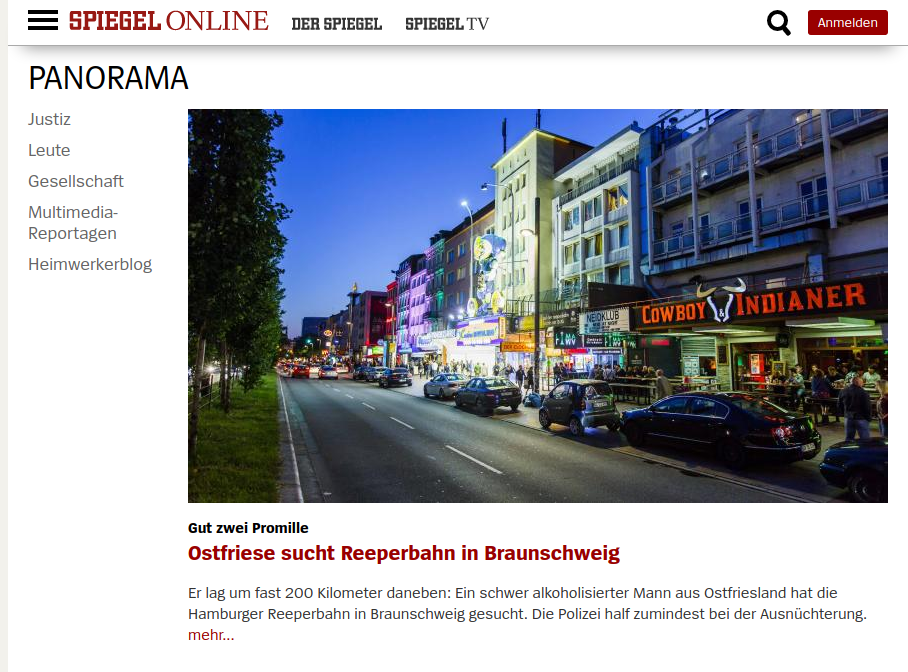
\includegraphics{img/human_readable.png}
\caption{Ein Artikel einmal in der normalen Darstellung\ldots{}}
\end{figure}

\end{no-prefix-figure-caption}

\begin{no-prefix-figure-caption}

\begin{figure}
\centering
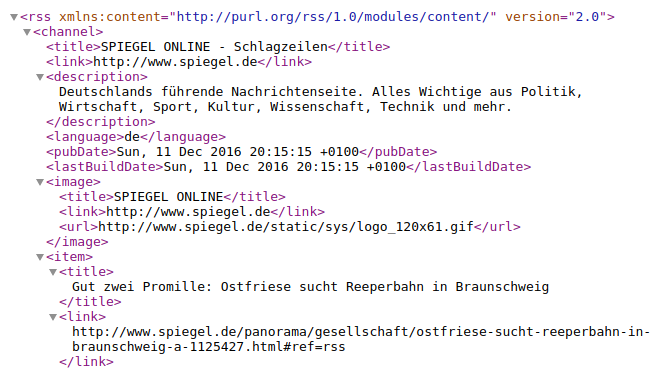
\includegraphics{img/rss.png}
\caption{\ldots{} und einmal als Teil eines RSS-Feeds}
\end{figure}

\end{no-prefix-figure-caption}

Diese Darstellung als RSS-Feed ermöglicht es, die Artikel verschiedener
Online-Zeitungen zu betrachten, ohne für jede Zeitung einen komplett
neuen Datensammler programmieren zu müssen.

Der letztendliche Datensammler ist ein Programm, welches ich in Python
geschrieben habe. Python ist eine Programmiersprache, die auf
Einfachheit und Flexibilität optimiert ist. Das Datensammelprogramm lädt
sich den RSS-Feed einer einzelnen Nachrichtenquelle periodisch herunter
und verarbeitet ihn weiter. Ich habe mich dazu entschieden, jeden
RSS-Feed alle 10s neu zu analysieren. Im ersten Schritt der Verarbeitung
lädt das Programm den Feed als Datei von den Servern der jeweiligen
Online-Zeitung herunter. Diese Datei ist eine sogenannte XML-Datei. In
ihr werden Daten als Baumstruktur abgebildet. Hierbei muss man sich die
Datei als ``Stamm'' des Baums vorstellen. Die ersten ``Äste'' der
Baumstruktur beinhalten die Metadaten, wie z.B. den Erstellungszeitpunkt
und den Herausgeber des Feeds. Die nachfolgenden ``Äste'' enthalten
jeweils einen Artikel. Diese Artikel wiederum beinhalten verschiedene
Unterelemente, d.h. die ``Äste'' verzweigen sich in weitere, kleinere
``Ästchen''. In diesen stehen nun z.B. der Autor des Textes, der Titel,
oder eben der eigentliche Inhalt des Textes. Diese textuelle
Repräsentation einer Baumstruktur gilt es nun in eine einfacher
verwendbare Repräsentation im Speicher des Python Programms umzuwandeln.
Hierfür wird eine Programmbiliothek verwendet, die einen sogenannten
XML-Parser beinhaltet, der genau dies erreicht. Nach diesem Schritt
können die einzelnen Artikel betrachtet werden. Hierbei wird zuallererst
überprüft, welche Artikel schon einmal verarbeitet wurden. Diese werden
verworfen. Die übriggebliebenen, also neuen Artikel werden in eine
allgemeinere Repräsentation für Neuigkeiten und ihre Metadaten gebracht,
die ich mir überlegt habe. Diese ist auch wieder eine Baumstruktur und
sieht aus wie in Abb. \ref{fig:ir}.

\begin{figure}
\centering
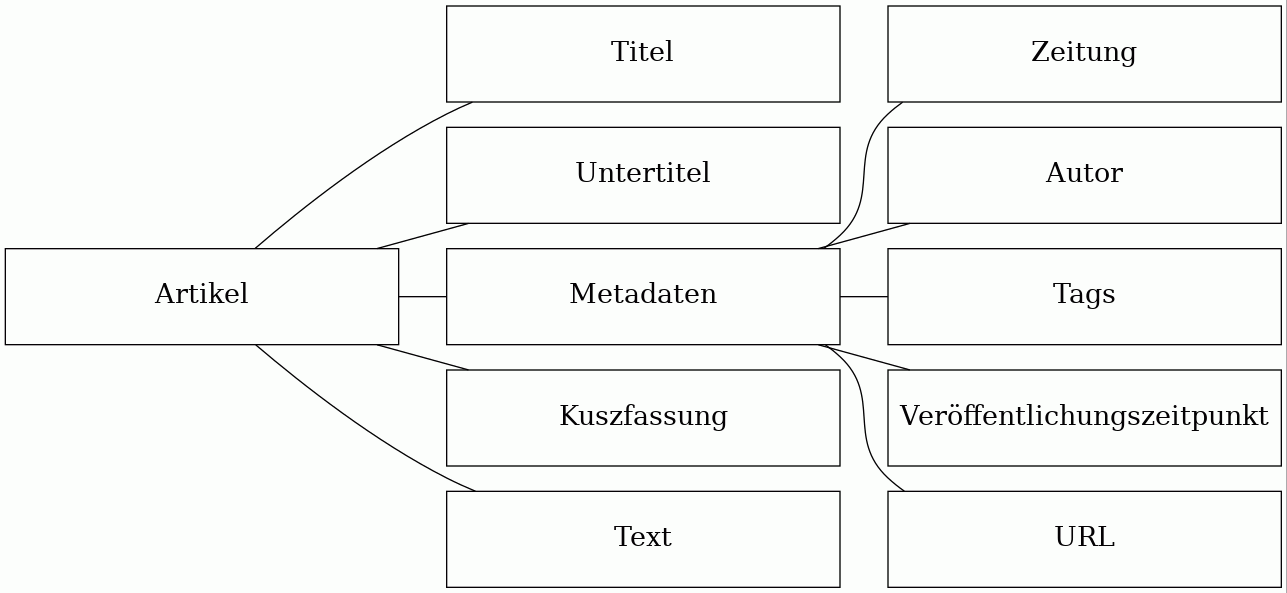
\includegraphics[width=7.00000cm]{img/ir.png}
\caption{Die Zwischenrepräsentation der Artikel\label{fig:ir}}
\end{figure}

\todo{find better visualisation}

Diese Umwandlung ist nötig, da der RSS-Standard zwar die grobe Struktur
und ihre Repräsentation als XML-Datei spezifiziert, letzten Endes jeder
Nachichtenanbieter allerdings doch nicht ganz kompatible Feeds
ausliefert. Diese kleinen Unterschiede werden hier also angeglichen,
damit die weitere Verarbeitung leichter vonstatten gehen kann, und in
der weiteren Verarbeitung keine Unterschiede mehr beachtet werden
müssen.

Ein weiteres Problem der RSS-Feeds ist, dass sie nur Kurzfassungen der
Artikel enthalten. In der Umwandlung müssen also noch die vollständigen
Artikel von der Internetseite des Nachrichtenanbieters heruntergeladen
und der Volltext aus dieser extrahiert werden. Hierzu wird zuerst das
HTML-Dokument der Seite ``geparsed''. Das Wort ``parsen'' ist sehr
schwierig ins Deutsche zu übersetzen. Es beschreibt den Sachverhalt, die
textuelle Repräsentation eines strukturierten Datensatzes in die
``native'' Repräsentation einer Programmiersprache für diesen Datensatz
zu bringen. Die ``native'' Repräsentation eines Datensatzes in einer
Programmiersprache ist die Standardform, diesen Datensatz abzubilden.
Diese hat oft bestimmte Funktionen, die das Programmieren vereinfachen,
wie z.B. die Zugriffsmöglichkeit auf einzelne Elemente bei Listen. Aus
dem ``geparsten'' HTML-Dokument werden nun die relevanten Teile, zu
denen z.B. nicht die Kopf- oder Fußzeile gehören, mithilfe sogenannter
``CSS-Selektoren'' identifiziert. Hiernach werden alle HTML-Elemente
dieser Bereiche in reinen Text umgewandelt.

Architektonisch ist der Datensammler ein Programm, in das weitere
kleinere Module ``hereingesteckt'' werden, die die einzelnen
Nachrichtenseiten ansprechen.

\begin{no-prefix-figure-caption}

\begin{figure}
\centering
\includegraphics{img/datensammler.png}
\caption{Der Datensammler und seine Module}
\end{figure}

\end{no-prefix-figure-caption}

\todo{adapt to actual used newspapers}

Am Ende der Datenaquirierung werden die gesammelten Daten an die nächste
Stufe weitergegeben, in der die Daten gespeichert werden.

\subsection{Speicherung}\label{speicherung}

Die nun gesammelten Daten müssen vor der weiteren Verwendung ersteinmal
strukturiert zwischenggespeichert werden. Dies geschieht in einer
Datenbank. Ich habe mich dafür entschieden, eine sogenannte
``NoSQL-Datenbank'' zu verwenden, da diese flexiblere Abfragemethoden
ermöglichen. ``NoSQL'' steht hierbei dafür, dass die Datenbank nicht
über die Datenbanksprache SQL angesprochen wird, wie es normalerweise
der Fall ist, sondern eine andere Abfragemöglichkeit bietet. Relativ
früh habe ich mich dafür entschieden, dass ich meine Datenbankabfragen
als ``MapReduce''-Funktionen formulieren möchte.

\subsection{MapReduce}\label{mapreduce}

Das MapReduce Verfahren hat einige große Stärken, wie z.B. die hohe
Parallelisierbarkeit und die damit verbundene hohe Geschwindigkeit, bei
gleichzeitig hoher Flexibilität. MapReduce ist ein von der Firma Google
eingeführtes Programmiermodell, welches wie folgt funktioniert:

\begin{no-prefix-figure-caption}

\begin{figure}
\centering
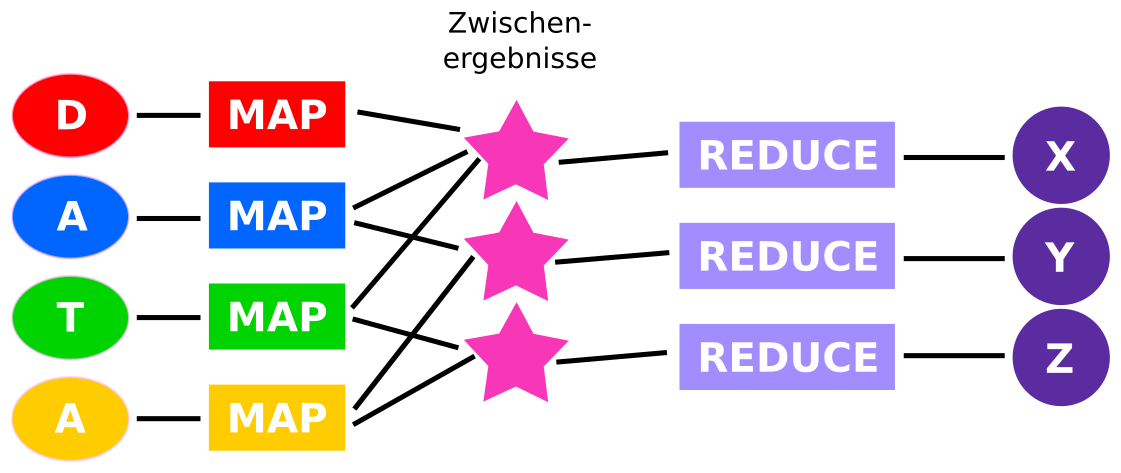
\includegraphics{img/MapReduce.png}
\caption{Der MapReduce prozess als Grafik}
\end{figure}

\end{no-prefix-figure-caption}

\begin{enumerate}
\def\labelenumi{\arabic{enumi}.}
\item
  Am Anfang des Prozesses steht eine Menge aus \(n\)
  Eingangsdatensätzen. In meinem Fall sind das die Zeitungsartikel, die
  als Objekte mit der oben beschriebenen Datenstruktur vorliegen. Für
  jeden dieser Artikel wird jetzt die Map-Funktion ausgeführt. Diese
  ordnet jedem Artikel \(n\) Schlüssel-Wert Paare zu. In dem Fall, dass
  wir zu jedem vorkommenden Wort die Häufigkeit bestimmen wollen, ordnet
  die Map-Funktion also jedem Artikel die Menge der darin enthaltenen
  Wörter zu. Da diese Funktion auf jeden Artikel angewandt wird, kann
  man sich in diesem Fall den gesammten Map-Prozess als eine Funktion
  vorstellen, die die Menge aller Artikel der Menge der darin
  enthaltenen Worte zuordnet. Der hierzu zugehörige Code einer map
  funktion ist:

\begin{lstlisting}
function map() {
  var text = this.text.replace(/[^A-Za-zÄäÖöÜüß ]/g, " ");   // entferne alle überfüssigen Satzzeichen, wie .,?!-
  var words = text.split(" ");   // Teile den text in Wörter
  for (var i = 0; i < words.length; i++) {   // für jedes Wort
        var word = words[i];
        if(word) {
           emit(word, 1);   // füge der Ausgabemenge das Wort hinzu
        }
  }
}
\end{lstlisting}

  \todo{make code great again!}
\item
  Im nächsten Schritt werden Elemente mit gleichen Schlüsseln gruppiert.
  Nach diesem Schritt liegt also eine Menge aus
  Schlüssel-Wertmengenpaaren vor (Auch wenn ich immer wieder das Wort
  Menge verwende, meine ich eigentlich Multimengen, da es relevent ist,
  wie oft ein bestimmtes Element in der Menge vorkommt
  \autocite{multimenge}). Dieser Schritt ist, anders als die anderen
  beiden Schritte, bei allen anderen Abfragen gleich. Da in unserem
  Beispiel das Wort als Schlüssel verwendet wurde, sähe eine
  beispielhafte Menge nach diesem Schritt wie folgt aus, was stark an
  eine Strichliste erinnert:

\begin{lstlisting}
[
   "der": {1; 1; 1; 1; 1; 1; 1; 1; 1},
   "die": {1; 1; 1; 1},
   ...
]
\end{lstlisting}
\item
  Im dritten und letzten Schritt wird für jeden Schlüssel die sogenannte
  Reduce-Funktion angewandt. Diese reduziert die Mengen, die den
  Schlüsseln zugeordnet sind, auf einen Wert. In unserem Beispiel fällt
  die Reduce-Runktion relativ einfach aus, da sie einfach nur die
  Elemente der Menge aufsummieren muss:

\begin{lstlisting}
reduce(key, values) {
  return values.reduce((previousValue, currentValue) => currentValue + previousValue);
}
\end{lstlisting}
\item
  Der vierte und letzte Schritt gehört eigentlich nicht mehr zum
  MapReduce-Verfahren. Dieser wird nach diesem ausgeführt und dient
  dazu, die Ergebisse zu sortieren und eventuell Feinheiten zu
  verbessern. So ist es zum Beispiel möglich, selten genutzte Worte oder
  sogenannte Stoppworte in diesem Schritt auszusortieren. Stoppworte
  sind häufig auftetende Worte, die keine Relevanz für die Erfassung des
  Dokumenteninhaltes haben. Hierfür verwende ich verschiedene
  Stoppwortlisten, die von Sprachforschern erstellt werden, zusammen mit
  eigenen Ergänzungen. Der hierzu gehörige Code, der die Wortliste
  filtert, sieht wie folgt aus:

\begin{lstlisting}
function filter(data) {
  return data.filter(word => stopwords.indexOf(word["_id"].toLowerCase()) < 0)
}
\end{lstlisting}

  Des weiteren wird in diesem Schritt versucht, Wörter mit dem gleichen
  Stamm, und somit mit der gleichen Bedeutung zusammenzuführen, auch
  wenn diese unterschiedliche Endungen haben. Ein Beispiel hierfür ist,
  das die Wörter ``Trump'' und ``Trumps'' zusammengezählt werden.
  Hierbei wird immer das kürzeste Wort behalten, da dies meist die
  Grundform ist.
\end{enumerate}

\subsection{Datenbank}\label{datenbank}

Nachdem klar war, wie die Abfragen formuliert werden sollten, habe ich
verschiedene Datenbanken in Betracht gezogen. Zuerst habe ich
angefangen, mit der Datenbank ``MongoDB'' zu arbeiten, störte mich aber
sehr stark an deren Komplexität. Außerdem bietet MongoDB keine
Möglichkeit, diese über das HTTP-Protokoll anzusprechen, was für die
Visualisierung allerdings sehr wichtig ist. Also sah ich mich nach
anderen Alternativen um und fand ``CouchDB'', welche vom Apache-Projekt
entwickelt wird. Diese Datenbank erfüllte die meisten meiner
Anforderungen relativ gut, weshalb ich meinen gesamten, bis dahin
existierenden Code an CouchDB anpasste. Nach einiger Zeit des Testens
stellte sich allerdings heraus, das CouchDB wahrscheinlich zu langsam
sein würde und ein unpassendes Rechteverwaltungssystem mitbringt, was
die Arbeitsersparnis im Gegensatz zu MongoDB zunichte machen würde. In
Folge dieser Erkentnis entschied ich mich dazu, meine Software zurück
auf MongoDB zu portieren und für diese eine HTTP-Schnittstelle zu
entwickeln.

\subsection{Middleware}\label{middleware}

Diese HTTP-Schnittstelle ist gewissermaßen das Bindeglied zwischen der
Datenbank und der Visualisierung, weshalb es im nachfolgenden
``Middleware'' genannt wird. Sie nimmt HTTP-Anfragen von der
Visualisierung (``Frontend'') entgegen, leitet diese an die Datenbank
weiter und schickt die Antwort der Datenbank an das Frontend zurück.
Insofern könnte man sie auch als Übersetzer zwischen verschiedenen
Protokollen verstehen. Eine Übersetzung ist notwendig, da ich die
Visualisierung im Webbrowser implementiert habe, und im Browser nur sehr
wenige Schnittstellen verfügbar sind. HTTP ist eine dieser wenigen
Möglichkeiten und bietet sich an, da es verhältnismäßig einfach zu
implementieren ist.

\subsection{Visualisierung}\label{visualisierung}

Ich habe mich entschieden, die Visualisierung im Browser umzusetzen.
Dies lag hauptsächlich daran, dass ich bereits einige der verwendeten
Technologien kannte, und somit die Einstiegshürde niedriger war.
Außerdem gibt es für den Browser und die damit verbundenen Technologien
bereits sehr gute Bibliotheken zur Datenvisualisierung, auf die ich für
meine Arbeit zurückgreifen konnte. Ein weiterer, nicht unwichtiger
Punkt, ist die einfache Portabilität von Programmen, welche im Browser
laufen: Sie können auf fast jedem Computer, unabhängig von
Betriebssystem oder Prozessorarchitektur, innerhalb von Sekunden
aufgerufen und ausgeführt werden.

Eines der Hauptziele bei der Konzeption und Entwicklung der gesamten
Analysesoftware war die Flexibilität: Es sollte möglichst schnell und
einfach möglich sein, verschiedene Analysen über den Datensatz
durchzuführen. Dies bezog sich nicht nur auf vorgefertigte, bei der
Entwicklung bedachte Analysen, sondern auch zukünftige Ansätze. So
sollte es einfach möglich sein, eigene neue Analysen über den Datensatz
durchzuführen. Dies führte zu der konzeptionellen Endscheidung, dass die
Analyse durch den Quellcode des Visualisierungsmoduls vorgegeben sein
sollte und alle anderen Zwischenschritte, wie die Middleware oder die
Datenbank nur auf die Anfragen des Analysemodul hören sollten. Dies hat
zur Folge, das ein großer Teil der Komplexität des Codes im Frontend
liegt.

Jede Visualisierung fragt am Anfang die benötigten Daten bei der
Middleware über MapReduce-Anfragen an. Die einzelnen Funktionen, die
hierzu benötigt werden, werden also in dem Code der Visualisierung
definiert und hängen davon ab, welche Daten aus dem Datensatz benötigt
werden. Dieser Vorgang kann mehrere Male wiederholt werden, um
verschiedene Informationen über verschiedene Aspekte des Datensatzes zu
bekommen. Hiernach werden die nun vorliegenden Daten weiterverarbeitet.
Sie können also gefiltert, sortiert oder miteinander verrechnet werden.
Liegen die Daten nun in der richtigen Form vor, kann die eigentliche
Visualisierung beginnen.

\todo{write about the actual visualisierung} * d3.js

\subsection{Zusammenführung}\label{zusammenfuxfchrung}

\todo{read} Da die Gesamte Software sehr modular aufgebaut ist, besteht
sie aus vielen kleinen Komponenten, die sehr spezialisiert und alleine
nicht sehr nützlich sind. Diese kleinen Komponenten nennt man in der
Softwareentwicklung ``Microservices''. Um aus diesen kleinen
Microservices eine funktionierende Software zu erhalten, muss man diese
jeweils in einer passenden Umgebung starten und richtig miteinander
verbinden. Um dies zu bewerkstelligen habe ich das Software-Paket
``Docker'' verwendet. Dieses erlaubt es zu aller erst die Einzelnen
Umgebungen für jeden Microservice zu beschreiben. Diese enthalten zum
Beispiel die Verschiedenen Programmbibliotheken, die ich in den
einzelnen Teilen verwandt habe, oder einen Webserver, um den
Visualisierungscode an den Webbrowser auszuliefern. Eine solche Umgebung
mit allen darin enthaltenen Programmen nennt man ``Container''. Diese
Container erstellt man immer auf der Basis eines anderen
Basiscontainers. Dies sorgt dafür, das man sich nicht immer um alles
innerhalb eines Containers kümmern muss, also zum Beispiel nicht immer
selber das Betriebssystem installieren muss, sondern nur noch die
eigenen Komponenten hinzufügen muss. Dies geschieht automatisiert über
eine Datei, die jedem Microservice bigefügt ist, dem sogenannten
``Dockerfile''. Auch ist es möglich komplett vorgefertigte Container zu
verwenden, was ich z.B. für die Datenbank nutze.

Die einzelnen Container, die nun die komplette Umgebung enthalten, die
die einzelnen Microservices zum laufen benötigen, müssen nun nur noch
alle richtig verbunden werden. dies Geschieht mit einem Programm namens
``Docker-compose''. Diesem gibt man eine Datei, die den zustand des
gesamten gewünschten Systems enthält. Automatisiert wird aus diesem und
allen Dockerfiles der Microservices dann genau dieses gewünschte System
erstellt und gestartet. Die Datei, die dieses System abbildet sieht wie
folgt aus:

\begin{lstlisting}
version: '2'

services:
   data-collectors:
      build: data-collectors/
      links:
         - mongodb
   backend:
      build: backend/
      links:
         - mongodb

   frontend:
      build: frontend/
      links:
         - backend
      ports:
         - "80:80"

   mongodb:
      image: "mongo:latest"
\end{lstlisting}

Auch hier sieht man wieder sehr schön die Struktur und die Modularität
der Software und ihre einzelnen Dienste.

Dieses System, das alle ständig laufenden Komponenten enthält, wird nun
auf einem Server gestartet und ermöglicht es sowohl den Code der
Visualisierung als auch Auskünfte über den Datensatz zu bekommen.

\section{Beobachtungen}\label{beobachtungen}

\subsection{Evaluation des Verfahrens}\label{evaluation-des-verfahrens}

\subsubsection{Ergebniss}\label{ergebniss}

\subsubsection{Technisch}\label{technisch}

\begin{itemize}
\tightlist
\item
  Map/Reduce bei jedem Query skaliert nicht :(
\end{itemize}

\subsection{Verschiedene Zeitungen im
Vergleich}\label{verschiedene-zeitungen-im-vergleich}

\section{Fazit}\label{fazit}

\section{Quellen}\label{quellen}

\todo{QUellen!!!}

\printbibliography

\end{document}
